\notechapter{N-20240727}{Hopf Fibration, Homotopy, and a Tempting Infinite-Stability Reading}

\section{The infinite-stability interpretation}

The line
\[
  0=1-1=-1+1=0
\]
invites an analytic and algebraic interpretation before its topological meaning is known.  The middle expressions suggest rearrangement, cancellation, and ambiguity of formal sums.  One tempting route is therefore
\[
\begin{array}{c}
  \text{alternating sums}\longrightarrow\text{regularization}\\
  \longrightarrow\text{Eilenberg swindle}\\
  \longrightarrow\text{vanishing under infinite stability.}
\end{array}
\]
This interpretation connects genuine mathematical mechanisms, but it ultimately points in the wrong direction.  The chapter develops it precisely enough that both its appeal and its failure become visible.

\section{The analytic reflex}

The most immediate association is the infinite alternating series
\[
  1-1+1-1+\cdots.
\]
Its partial sums are
\[
  1,\ 0,\ 1,\ 0,\ \ldots,
\]
so the ordinary limit does not exist.

\begin{definition}[Ces\`aro summation]
Let \(s_n=a_0+\cdots+a_n\) be the partial sums of a series.  If the averages
\[
  \sigma_N=\frac{s_0+s_1+\cdots+s_N}{N+1}
\]
converge to \(L\), then the series is Ces\`aro summable to \(L\).
\end{definition}

For the alternating series, the Ces\`aro averages of the partial sums tend to
\[
  \frac12.
\]
Thus the expression is not convergent in the usual sense, but it has a regularized value in the Ces\`aro sense.

\begin{definition}[Abel summation]
Given a formal series \(\sum_{n\ge0}a_n\), form its power series
\[
  F(r)=\sum_{n\ge0}a_nr^n
\]
for \(0<r<1\).  If \(F(r)\) has a limit \(L\) as \(r\to1^-\), then the original series is Abel summable to \(L\).
\end{definition}

For
\[
  1-1+1-1+\cdots,
\]
one has
\[
  1-r+r^2-r^3+\cdots=\frac{1}{1+r},
\]
so Abel summation again gives \(1/2\).

\begin{remark}
The same cultural memory also points toward the analytic continuation of the Dirichlet eta function.  The important point is not the exact analytic formalism, but the habit of reading a formally divergent expression through a more flexible rule.
\end{remark}

This motivates reading the line
\[
  0=1-1=-1+1=0
\]
as a statement about how formal algebra changes when one passes from finite arithmetic to limiting procedures.  In ordinary arithmetic, the line is trivial.  In the world of infinite expressions, however, the order of grouping and the rule of interpretation may change what the expression seems to mean.

\begin{claim}[Analytic slogan]
The equation should perhaps be read not as a numerical equality, but as evidence that cancellation becomes unstable once infinite formal processes are allowed.
\end{claim}

\section[Why Hopf and K-theory require more than summation]{Why Hopf and \(K\)-theory require more than summation}

The analytic interpretation alone did not explain why the meme included the Hopf fibration and \(K\)-theory.  Those are not the usual tools for assigning values to divergent series.  The Hopf fibration suggests homotopy and stable phenomena.  \(K\)-theory suggests addition, cancellation, and group completion of mathematical objects.

The analytic reflex therefore has to be upgraded.  Instead of asking only whether
\[
  1-1+1-1+\cdots
\]
has a regularized value.  The relevant question is whether a categorical or \(K\)-theoretic setting can make cancellation legitimate through infinite size or stability.

That is exactly the kind of situation where the Eilenberg swindle appears.

\section{The Eilenberg swindle as the central candidate}

The Eilenberg swindle is the mechanism that made the analytic reflex look relevant to \(K\)-theory.

\begin{theorem}[Eilenberg swindle, working form]
Suppose an additive category has countable direct sums and an object
\[
  S=A\oplus A\oplus A\oplus\cdots.
\]
Then
\[
  S\cong A\oplus S.
\]
Consequently, any Grothendieck-type invariant \(K_0\) compatible with direct sums satisfies
\[
  [S]=[A]+[S],
\]
and therefore forces
\[
  [A]=0.
\]
\end{theorem}

\begin{proof}[Idea]
The isomorphism is the shift of the infinite direct sum:
\[
  A\oplus A\oplus A\oplus\cdots
  \cong
  A\oplus(A\oplus A\oplus A\oplus\cdots).
\]
The finite summand \(A\) is absorbed by the infinite tail.  Passing to an additive invariant converts this absorption into a vanishing statement.
\end{proof}

This is the algebraic counterpart of the alternating-series picture.  One can group an infinite expression in different ways:
\[
  (1-1)+(1-1)+\cdots=0,
\]
but also
\[
  1+(-1+1)+(-1+1)+\cdots=1.
\]
The paradox is not that arithmetic is broken.  The point is that infinite formal manipulation can erase the distinction between adding one copy and adding no copy, because the tail of the expression absorbs the finite change.

\begin{remark}
This makes the line \(0=1-1=-1+1=0\) look like a compact symbolic form of infinite absorption.  The two middle expressions are different finite presentations, but in an infinitely stable setting they may collapse to the same zero class.
\end{remark}

\section[How the swindle resembles a K-theory statement]{How the swindle resembles a \(K\)-theory statement}

In algebraic \(K\)-theory, one often begins with a category of objects equipped with a direct-sum operation.  The first invariant records formal additive differences.

\begin{definition}[Grothendieck group]
Let \(M\) be a commutative monoid.  Its Grothendieck group \(K_0(M)\) is the universal abelian group receiving a monoid homomorphism from \(M\).  Concretely, elements may be represented by formal differences
\[
  [A]-[B],
\]
subject to the relation
\[
  [A\oplus C]-[B\oplus C]=[A]-[B].
\]
\end{definition}

The expression \(1-1\) then resembles a formal difference between one positive copy and one negative copy.  The Eilenberg-swindle interpretation proposes that a sufficiently infinite environment can force such formal differences to vanish.

\begin{proposition}[Vanishing by absorption, heuristic form]
If a category contains an object \(S\) with
\[
  S\cong S\oplus A,
\]
then any additive invariant that sees direct sum as addition tends to identify the class of \(A\) with zero.
\end{proposition}

This is why swindle arguments prove vanishing theorems in categories with infinite coproducts or infinite-dimensional stabilization.  At the level of intuition, the resulting chain is: Hopf fibration points toward stable homotopy; stable homotopy points toward group completion in K-theory; group completion suggests infinite stability and the Eilenberg swindle; the final line is read as symbolic infinite cancellation.
In this interpretation, the final line is an extreme arithmetic trick: after enough stabilization, the complicated machinery collapses into the fact that infinity can absorb a finite summand.

\section{The role assigned to the Hopf fibration}

Within this interpretation, the Hopf fibration serves as the geometric entrance into stable homotopy.  The Hopf map
\[
  S^3\to S^2
\]
is a concrete example of a map whose nontriviality is not visible from ordinary dimension-counting.  It teaches that topology can remember a hidden process.

From there, stable homotopy suggests that some phenomena persist after suspending or stabilizing.  The tempting analogy connects this with the word ``stable'' in algebra: after passing to a sufficiently stabilized category, hidden structure might become algebraic cancellation and ultimately a vanishing statement.

This is not a precise theorem, but a ladder of associations:
\[
  \text{Hopf}\quad\rightsquigarrow\quad
  \text{stable homotopy}\quad\rightsquigarrow\quad
  \text{stable algebra}\quad\rightsquigarrow\quad
  \text{swindle}.
\]
As a heuristic, it makes the sequence of clues less arbitrary.  The Hopf fibration stood for the beginning of stable topology; the equation stood for the end of a stabilization trick.

\section{The meme as an association ladder}

The diagram should not be read as a proof.  It is a ladder of associations linking elementary cancellation to progressively more structural interpretations.

\Needspace{18\baselineskip}
\begin{figure}[htbp]
  \centering
  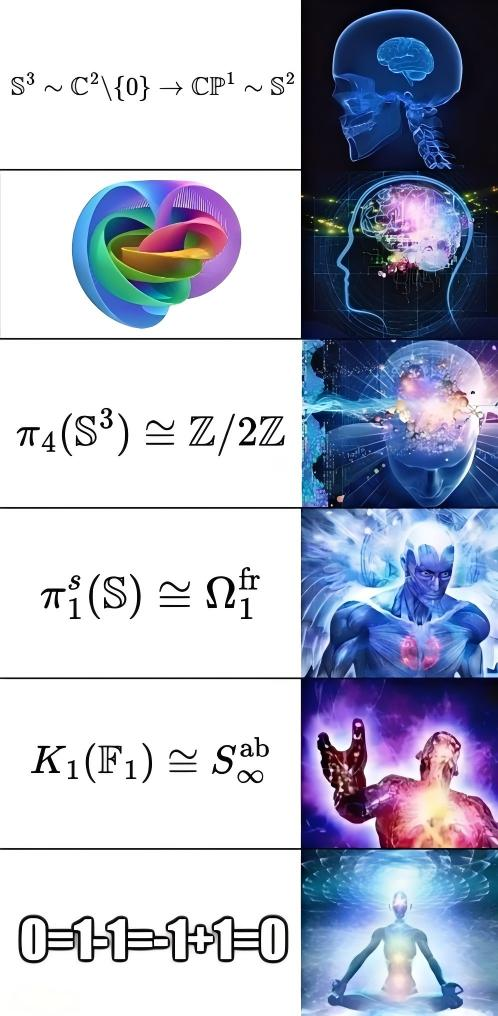
\includegraphics[width=0.58\textwidth]{figures/N-20240727/hopf_meme.jpg}
  \caption{The meme that compressed Hopf fibration, stable homotopy, \(K\)-theory, and the equation \(0=1-1=-1+1=0\) into one ladder.}
\end{figure}

Under the infinite-stability interpretation, the ladder becomes a sequence of working meanings.  The Hopf fibration represents hidden topology; homotopy groups record deformation; stable homotopy records persistence under stabilization; \(K\)-theory organizes addition and cancellation; and the Eilenberg swindle produces vanishing through infinite absorption.
The interpretation is therefore more than a random guess about divergent series: it reconciles the visible clues with a genuine mechanism in \(K\)-theory.

\section{The infinite-stability thesis}

The interpretation can be stated cleanly as a working thesis.

\begin{theorem}[Infinite-stability interpretation]
In elementary arithmetic, \(0=1-1=-1+1=0\) is trivial.  In an infinitely stable categorical setting, however, finite additions and cancellations can be absorbed by an infinite tail.  The Eilenberg swindle expresses this absorption.  Therefore the equation may be read as a symbolic way to say that certain \(K\)-theoretic invariants vanish once infinite direct-sum operations are allowed.
\end{theorem}

This reading emphasizes three words:
\[
\begin{array}{c}
\text{infinity,}\
\text{stability,}\
\text{vanishing.}
\end{array}
\]
The line \(0=1-1=-1+1=0\) then becomes an emblem of the idea that a sophisticated invariant may collapse because the ambient category is too large.

\section{Where the interpretation fails}

The weakness is now visible.  The relevant construction uses finite sets, configuration spaces, and the Hopf fibration, while the swindle explanation relies heavily on infinite objects.  The analytic examples likewise use infinite series and limiting procedures.  The interpretation points toward the right vocabulary but not the correct object.

Even so, the interpretation captures several genuine connections:
\begin{itemize}
  \item alternating sums explain why \(1-1\) and \(-1+1\) feel like more than ordinary arithmetic;
  \item the Eilenberg swindle explains how infinite stabilization can trivialize \(K\)-theoretic information;
  \item \(K\)-theory really is about direct sum, group completion, and cancellation;
  \item the Hopf fibration really does point toward stable homotopy.
\end{itemize}

The central claim is not that \(0\) is secretly nonzero.  It is that in an infinitely stabilized algebraic world, the distinction between adding and not adding a finite piece can disappear.  This explains a real vanishing mechanism, but not the finite homotopical loop represented by the equation.
